%!TEX root = stoh_modeling.tex
\section{Результаты}
\subsection{Описание реакций}
Опишем реакции для одного ядра (для остальных ядер аналогично). Для каждого сайта присоединения реакции присоединения и отсоединения будут
иметь одинаковый вид. Основным отличием будет какой именно ТФ присоединяется/отсоединяется. Для активаторов (в нашей работе это \textbf{cad}
или \textbf{bcd}) реакции примут следующий вид:
\begin{align*}
N^{unbound}   \xrightarrow{C_i \cdot N^{unbound}} & N^{binded} + A\\
N^{binded} + A \xrightarrow{C_i \cdot N^{binded}}  & N^{unbound}
\end{align*}

Для репрессоров реакции будут выглядеть так:

\begin{align*}
N^{unbound}   & \xrightarrow{C_i \cdot N^{unbound}} N^{binded} + R\\
N^{binded} + R &  \xrightarrow{C_i \cdot N^{binded}}  N^{unbound}
\end{align*}
где $C_i$ - коэффициент присоединения к $i$-ому сайту, $R$ - количество репрессоров и $A$ - количество активаторов.

Теперь запишем реакции транскрипции и трансляции:

\begin{align*}
\varnothing \xrightarrow{p_{\lambda} \cdot p_{\alpha}^{A} \cdot p_{\beta}^{R}} mRNA \\
mRNA \xrightarrow{p_{\gamma} \cdot mRNA} N^{unbound} \\
\end{align*}

где $p_{\lambda}$, $p_{\alpha}$, $p_{\beta}$, $p_{\gamma}$ - коэффициенты транскрипции, активации, регрессии и трансляции соотвественно.

Реакции деградации:

\begin{align*}
mRNA \xrightarrow{p_{\theta} \cdot mRNA} \varnothing \\
N^{unbound} \xrightarrow{p_{\phi} \cdot N^{unbound}} \varnothing \\
\end{align*}
где $p_{\theta}$, $p_{\phi}$ - коэффициенты деградации мРНК и белка соотвественно.

Так же нужно учесть диффузию - перетекание белка в соседние ядра:

\begin{align*}
N_i   \xrightarrow{p_{\xi} \cdot max(N_i - N_{i+1}, 0)} & N_{i+1} \\
N_i   \xrightarrow{p_{\xi} \cdot max(N_i - N_{i-1}, 0)} & N_{i-1}
\end{align*}
где $p_{\xi}$ - параметр диффузии, $i$ - номер ядра.
В результате наша модель имеет 7 параметров - $p_{\lambda}$, $p_{\alpha}$, $p_{\beta}$, $p_{\gamma}$, $p_{\theta}$, $p_{\phi}$, $p_{\xi}$.


\subsection{Разработка программного обеспечения}
Пакет был разделён на четыре компоненты:
\begin{itemize}
  \item Генерация системы реакций для пакета StochKit с помощью языка программирования Python
  \item Стохастическое моделирование с помощью пакета StochKit
  \item Оптимизация параметров модели с помощью DEEP
  \item Анализ результатов с помощью языка программирования R
\end{itemize}

Основной трудностью было наладить работу DEEP совместно с StochKit. Для этого нужно было изменить исходники StoсhKit, чтобы после каждого запуска он выводил ошибку моделирования при заданных параметрах.

\subsection{Анализ результатов}
В силу ограниченности возможности работы на кластере, было произведено несколько стартов. Было построены графики зависимости
концентрации белка \textbf{kni} от ядра к концу моделирования (в нашем случае это 60 минута).
\begin{figure}[h]
 	\center{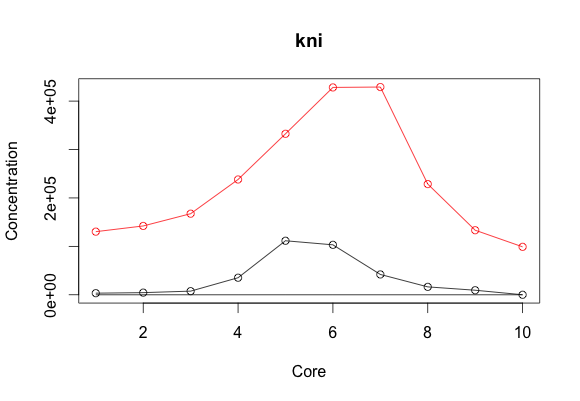
\includegraphics[width=1\linewidth]{kni}}
  \caption{Зависимость концентрации белка kni от ядра. Чёрным цветом - результат моделирования, красный цвет - экспериментальный расчёты}
  \label{fig:kni}
\end{figure}

\begin{figure}[h]
 	\center{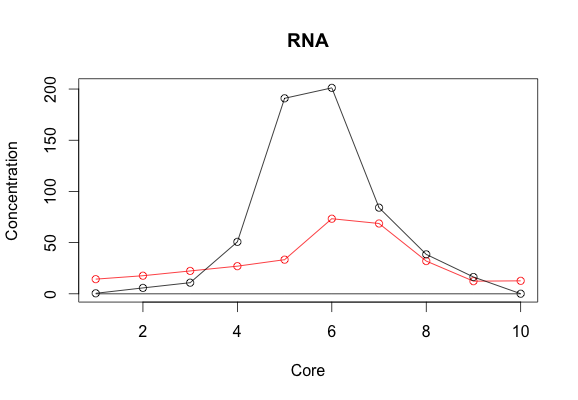
\includegraphics[width=1\linewidth]{rna}}
  \caption{Зависимость концентрации мРНК от ядра. Чёрным цветом - результат моделирования, красный цвет - экспериментальный расчёты}
  \label{fig:rna}
\end{figure}

На графиках (\ref{fig:kni}, \ref{fig:rna}) отчётливо видно, что поведение концентраций у белка \textbf{kni} и мРНК схожи с экспериментальными расчётами.
